%-----------------------------------------------------------------------------------------------
% 2020-NaaktgeborenC-PolyProc.tex - by C. Naaktgeboren
% License: CC-BY-NC-ND 4.0 - https://creativecommons.org/licenses/by-nc-nd/4.0/
%-----------------------------------------------------------------------------------------------
\documentclass[fleqn,11pt]{SelfArx}
%-----------------------------------------------------------------------------------------------
\usepackage[greek,french,english]{babel}
\usepackage[squaren,cdot]{SIunits}
\usepackage{amsthm}
\usepackage{CormorantGaramond}
%-----------------------------------------------------------------------------------------------
\newcommand{\parxyz}[3]{\left(\frac{\partial {{#1}}}{\partial {{#2}}}\right)_{\!\!\!{#3}}}
\newcommand{\inlxyz}[3]{({\partial {{#1}}}/{\partial {{#2}}})_{{#3}}}
\newcommand{\bri}[2]{(\partial {{#1}})_{{#2}}}
%-----------------------------------------------------------------------------------------------
\newcommand{\GRtxt}[1]{\begin{otherlanguage}{greek}{{#1}}\end{otherlanguage}}
\newcommand{\FRtxt}[1]{\begin{otherlanguage}{french}{{#1}}\end{otherlanguage}}
%-----------------------------------------------------------------------------------------------
\setlength{\abovecaptionskip}{4pt}
\setlength{\columnsep}{5.5mm}
\setlength{\columnseprule}{0.2pt}
\setlength{\fboxrule}{0.4pt} % Width of the border around the abstract
%-----------------------------------------------------------------------------------------------
\definecolor{color1}{RGB}{0,0,90} % Color of the article title and sections
\definecolor{color2}{RGB}{0,20,20} % Color of the boxes behind the abstract and headings
\definecolor{color3}{RGB}{0,0,192} % Color of the article title and sections
%-----------------------------------------------------------------------------------------------
\usepackage[hyperindex,breaklinks]{hyperref} % Required for hyperlinks
\hypersetup{%
    hidelinks,
    colorlinks,
    breaklinks=true,
    urlcolor=color3,
    citecolor=color1,
    linkcolor=color1,
    bookmarksopen=false,
    pdftitle={Title},
    pdfauthor={Author}
}
%-----------------------------------------------------------------------------------------------
\newtheorem{theorem}{Theorem}
\newtheorem{definition}{Definition}
\newtheorem{example}{Example}
\newtheorem{lemma}{Lemma}
\newtheorem{conjecture}{Conjecture}
\newtheorem{proposition}{Proposition}
%-----------------------------------------------------------------------------------------------
\makeatletter
\immediate\write18{datelog > \jobname.info}
\makeatother
%-----------------------------------------------------------------------------------------------
% Journal information
\JournalInfo{Preprints Server Name} % TODO: Update-me
\Archive{Compiled on \input{\jobname.info}}
% Article title
\PaperTitle{On Exact and Local Polytropic Processes: Etymology, Modeling, and Requisites}
\Authors{C.~Naaktgeboren\textsuperscript{1$\star$}}
\affiliation{\textsuperscript{1}\textit{Universidade Tecnológica Federal  do  Paraná  --  UTFPR,
Câmpus Guarapuava. Grupo de Pesquisa em Ciências Térmicas.}}
\affiliation{\textsuperscript{$\star$}\textbf{Corresponding  author}:
NaaktgeborenC$\cdot$PhD@gmail$\cdot$com}
\Keywords{Thermodynamics --- Polytropic Processes --- Logical Processes --- Etymology}
\newcommand{\keywordname}{Keywords}
\Remarks{%
    Provides \emph{etymology} for the `polytropic' term ---
    Defines \emph{logical thermodynamic process} ---
    Defines \emph{exact polytropic process} ---
    Presents a statement for \emph{local polytropic process} ---
    Defines theoretical \emph{requisites} for exact polytropic process
}
\newcommand{\remarkname}{Remarks}
%-----------------------------------------------------------------------------------------------
\Abstract{%
    This preprint concerns polytropic processes,  a  fundamental  process  type  in  engineering
    thermodynamics. An etymology is presented for the term, and the ties to its  usefulness  are
    identified. The seemingly new support concept of `logical' thermodynamic process, as well as
    the seemingly new working concept  of  `exact'  polytropic  process,  and  a  statement  for
    `local' polytropic  process,  are  herein  provided.  The  proposition  of  employing  local
    polytropic  processes  as  computational   discrete   elements   for   generic   engineering
    thermodynamics process modeling is made. Finally, theoretical requisites for a process to be
    an exact polytropic one, including the deduction of the most general equation  of  state  of
    the underlying substance, are discussed beyond a reference.
}
%-----------------------------------------------------------------------------------------------
\begin{document}
%-----------------------------------------------------------------------------------------------

\thispagestyle{empty}

\flushbottom

\maketitle

%-----------------------------------------------------------------------------------------------
\section*{License}

    \scriptsize\noindent%
    \begin{minipage}{\columnwidth}
        \centering\tt
        \includegraphics[height=6.0mm]{cc/by-nc-nd.pdf}\\[0.5\smallskipamount]
        {\scriptsize\url{https://creativecommons.org/licenses/by-nc-nd/4.0/}}
    \end{minipage}
    \normalsize

%-----------------------------------------------------------------------------------------------

\tableofcontents

%-----------------------------------------------------------------------------------------------
\section{Introduction}\label{sec:introduction}

    Many equilibrium engineering thermodynamics processes  are  taken  to  follow  a  polytropic
    relationship,
    %
    \begin{equation}
        Pv^n = \mathsf{c} = \mbox{const.},
        \label{eq:poly}
    \end{equation}
    %
    \noindent in which $P$ is the system pressure, usually in \kilo\pascal, $v$  is  the  system
    specific volume, usually in $\meter\cubed\!\per\kilogram$,  and  $n$  is  the  dimensionless
    polytropic exponent~\cite{2013-CengelYA+BolesMA-AMGH}---which, for a  `1--2'  process,  with
    initial and final end states labeled as `1' and `2', can also be written  in  terms  of  end
    state properties, as $P_1v_1^n = P_2v_2^n$, which also sets  the  particular  value  of  the
    $\mathsf{c}$ constant.

    Some mainstream thermodynamics textbooks introduce polytropic processes in  the  context  of
    closed system boundary work, as a $P\!:\!P(v)$ relationship to plug into the  boundary  work
    integral,   which    contains    a    $P\,dv$    integrand~\cite{2013-CengelYA+BolesMA-AMGH,
    2002-MoranMJ+ShapiroHN-LTC, 1985-WylenG-Wiley}. In such texts, the  polytropic  relationship
    is frequently said to find support in measurements, while no specific theoretical derivation
    is presented at the point of introduction.

    On  the  other  hand,  other  texts~\cite{1986-JonesJB+HawkinsGA-Wiley,   2006-BejanA-Wiley,
    2015-KroosKA+PotterMC-Cengage} include derivations that lead to a polytropic process, or  at
    least to an isentropic version of it, in which the exponent $n$ has a determined value.

    Moreover, Bejan~\cite[p.~175]{2006-BejanA-Wiley} indicates that a constant  $Pv^n$  relation
    only holds \emph{locally} if the process is such that $n$ is a function of either $P$,  $v$,
    or both.

    A paper due to Christians~\cite{2012-ChristiansJ-IntJMechEngEduc} discusses the topic from a
    perspective  of  teaching  polytropic  processes  themselves,  placing   emphasis   on   the
    \emph{heat-to-work transfer ratio}---named by that author as ``energy transfer ratio''---and
    how its constancy not only yields, but constitutes  a  prerequisite  for  a  process  to  be
    polytropic, besides, naturally, the constancy of the caloric properties of the working  pure
    substance.

    Starting with  an  \emph{etymological}  presentation  of  polytropic  processes,  this  work
    proposes and develops the concepts of \emph{exact polytropic}  and  \emph{local  polytropic}
    processes, as well as the supporting concept of \emph{logical thermodynamic} processes,  and
    presents theory-derived \emph{requisites} for a process  to  be  exactly  polytropic  beyond
    reference~\cite{2012-ChristiansJ-IntJMechEngEduc}. Moreover, local polytropic processes  are
    proposed as discrete building blocks for general  engineering  thermodynamics  \emph{process
    modeling}.

%-----------------------------------------------------------------------------------------------
\section{Etymology of the `Polytropic' Term}\label{sec:etymology}

    The `polytropic' term has its etymology  (origin)  in  the  Greek  language.  This  author's
    sources   on   Greek   are   mostly   based   on   modern   romance   languages,   such   as
    French~\cite{1968-Chantraine-Klincksieck,    2000-BaillyA-Hachette}    and    his     native
    Portuguese~\cite{1997-ManiatoglouMPF-Porto}; therefore, the etymology herein  brought  forth
    will include intermediate French terms.

    The word `polytropic' stems  from  the  Greek  word  `\GRtxt{pol'utropoc}'  that  itself  is
    composed of  two  Greek  words:  (i)~`\GRtxt{pol'uc}'\footnote{The  lexical  form  of  Greek
    adjectives is the nominative, singular, masculine. The nominative,  singular,  \emph{neuter}
    of `\GRtxt{pol'uc}' is `\GRtxt{pol'u}'.}, and (ii)~`\GRtxt{tr'opoc}'.

    The  Greek  adjective  `\GRtxt{pol'uc}'  includes  meanings  such  as  \FRtxt{\og  abondant,
    nombreux,   vaste   \fg}~\cite{1968-Chantraine-Klincksieck},   i.e.,   abundant,   numerous,
    vast~\cite{2009-BarrierMA+ViviesC-Auzou,  2011-SilvaASM-WMFMartinsFontes}.  The  Greek  noun
    `\GRtxt{tr'opoc}'   includes   meanings   such   as   \FRtxt{\og   manière,   façon,    mode
    \fg}~\cite{2000-BaillyA-Hachette},      i.e.,      manner,      way,      fashion,       and
    mode~\cite{2009-BarrierMA+ViviesC-Auzou,  2011-SilvaASM-WMFMartinsFontes}---hence,  meaning:
    numerous forms, or many ways.

    The composed Greek noun `\GRtxt{pol'utropoc}'  is  also  lexical,  and  includes  figurative
    meanings such as \FRtxt{\og souple, habile,  industrieux  \fg}~\cite{2000-BaillyA-Hachette},
    i.e., flexible, adaptive, able, laborious~\cite{2011-SilvaASM-WMFMartinsFontes}; as well  as
    meanings    such    as    \FRtxt{\og    versatilité,     très     divers,     très     varié
    \fg}~\cite{2000-BaillyA-Hachette}, i.e., versatility, very diverse, a  great  variety---thus
    indicating the \emph{wide-range} of processes that it is capable of representing.

    In  fact,  from  a  mathematical  standpoint,  Equation~(\ref{eq:poly}),  there  are  really
    infinitely many allowable (possible) values for the real polytropic exponent $n$ and for the
    $\mathsf{c}$ constant; thence, uncountably many processes departing  from  uncountably  many
    initial states. It is this kind of flexibility that is  encoded  in  the  etymology  of  the
    process name.

%-----------------------------------------------------------------------------------------------
\section{Exact and Local Polytropic Processes}\label{sec:exact.poly}

    %---------------------------------------------------------------------------------------
    \subsection{Logical Processes}\label{sec:logical}

    In equilibrium engineering thermodynamics, a \emph{process}---more properly  a  quasi-static
    or quasi-equilibrium one---is defined in terms of changes from a certain  equilibrium  state
    of a system to another~\cite{2013-CengelYA+BolesMA-AMGH}, with process \emph{path} being the
    (infinite) sequence of (quasi-)equilibrium states visited by the system during the  process.
    A process can be referred to by its path, with implicit or explicit end states.

    It is worth noting that no constraints are stated for the end states of  a  process  in  its
    definition.  This  allows  for  the  needed  flexibility  in  describing  the   variety   of
    transformations systems and control volumes can undergo in engineering thermodynamics.

    This lack of end state constraints in the definition of a process allows them to be splitted
    into multiple, successive `sub-processes' that still fit the definition  of  a  process,  as
    well as to merge multiple successive ones together into `super-processes' that also fit  the
    definition of a process. This ability is extremely useful in grouping and splitting  systems
    and control volumes along with their underlying processes---a common practice in engineering
    thermodynamics.

    However, in order to make the intended distinction  between  proposed  `exact'  and  `local'
    polytropic processes, additional constraints need to be made to process  end  states.  Thus,
    the following defines a \emph{logical  thermodynamic  process},  which  is  a  thermodynamic
    process with constrained end states. In  context,  i.e.,  in  thermodynamics  texts,  what's
    defined next can be simply called a `logical process':

    \begin{definition}[logical process]\label{def:logical.proc}
        A logical process is one in which its stated defining conditions, which  determines  all
        of the allowed interactions or property relations for the underlying system  or  control
        volume, uniformly and continually apply to the  entirety  of  its  path  from---but  not
        earlier than---its initial state until---but not later than---its end state.
    \end{definition}

    Therefore,  for  a  simple  compressible  system---one  admitting   only   work   and   heat
    interactions---either stated heat and work interactions, or system property  specifications,
    or combinations of the two, define possible logical processes.

    Moreover, the stated defining conditions of a logical process can  also  carry  a  `logical'
    qualifier, as to make it explicit they're being used in the definition of a logical process,
    as in the `logical conditions,' or `defining logical conditions'  expressions.  Furthermore,
    the conditions themselves can carry the `logical' qualifier, for the same purpose.

    \begin{example}\label{ex:ideal.Diesel}
        The   well-known   air-standard   ideal   Diesel    power    cycle,    illustrated    on
        Figure~\ref{fig:cycle.Diesel}, with `intake' state (of lowest temperature  and  pressure
        and maximum specific volume) labeled as `1', can be divided in different ways using only
        logical processes. One such division is: (i)~`logical isentropic compression',  ($\Delta
        s\!=\!0 \therefore Q\!=\!0$, $W\!\!<\!0$), (ii)~`logical isobaric heating',  ($Q\!>\!0$,
        $\Delta P\!=\!0 \therefore W\!\!>\!0$), (iii)~`logical isentropic  expansion',  ($\Delta
        s\!=\!0  \therefore  Q\!=\!0$,  $W\!\!>\!0$),  and  (iv)~`logical  isochoric   cooling',
        ($Q\!<\!0$, $\Delta v\!=\!0 \therefore W\!\!=\!0$), which correspond,  respectively,  to
        the `1--2', `2--3', `3--4', and `4--1' processes, i.e., to the canonical  processes  for
        this cycle, excluding sub-processes thereof. Another possible division is:  (a)~`logical
        isentropic   compression',   ($\Delta   s\!=\!0   \therefore   Q\!=\!0$,   $W\!\!<\!0$),
        (b)~`logical   no-heat-removal   expansion',   ($Q\!\geqslant\!0$,   $W\!\!>\!0$),   and
        (c)~`logical isochoric cooling', ($Q\!<\!0$,  $\Delta  v\!=\!0  \therefore  W\!\!=\!0$),
        which correspond,  respectively,  to  the  `1--2',  `2--4'  (through  `3'),  and  `4--1'
        processes, excluding sub-processes thereof, since these encompass  the  farthermost  end
        states that uniformly and continually match the stated defining logical conditions  (a),
        (b), and (c).
    \end{example}

    \begin{figure}[ht]
        \centering
        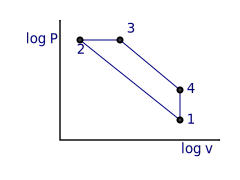
\includegraphics[width=40mm]{fig/idealDieselExample.pdf}
        \caption{Air-standard ideal Diesel cycle in $\log  P  \times  \log  v$  coordinates,  in
            support for the Example~\ref{ex:ideal.Diesel}.}
        \label{fig:cycle.Diesel}
    \end{figure}

    %---------------------------------------------------------------------------------------
    \subsection{Exact Polytropic Processes}\label{sec:exact}

    One is now in a position to define \emph{exact polytropic processes}:

    \begin{definition}[exact polytropic process]\label{def:exact.poly.proc}
        An exact polytropic process is a  logical  process  in  which  either  (i)~a  polytropic
        relation $Pv^n = \mbox{const.}$, with a  unique  polytropic  exponent  $n$,  or  (ii)~an
        isochoric logical condition, can be its sole logical defining condition,  provided  that
        no state in its path is visited more than once or serves simultaneously as  initial  and
        final end states in a given execution.
    \end{definition}

    It is worth noting that isochoric processes are equivalent to polytropic processes  with  $n
    \to \pm\infty$ between stated end states. Definition~\ref{def:exact.poly.proc} accounts  for
    the isochoric process non-unique polytropic exponent by explicitly including it as  a  valid
    exact polytropic process.

    \begin{lemma}\label{lemm:no.reversal}
        Any logical process defined by a single polytropic relation  with  a  unique  polytropic
        exponent, with non-identical end states can only be an exact polytropic process  in  the
        absence of reversals in its path.
    \end{lemma}

    \begin{proof}
        Let a logical process $\mathcal{P}_{1,2}$ be defined by  a  single  polytropic  relation
        with a unique polytropic exponent $n$, with non-identical end  states  `$1$'  and  `$2$'
        that contains a set of reversal states `$r_i$', with $\{ i \in \mathbb{Z} | i  \geqslant
        1 \}$ in its path.

        Without loss of generality, let further $P_{r_1}  <  P_1$,  if  $n  \neq  0$,  i.e.,  an
        initially pressure-decreasing process---since the following argument  can  be  otherwise
        flipped, or laid out in either direction in $v$, for non-zero $n$:

        Let state `$\epsilon$', defined as $(P_{\epsilon}, v_{\epsilon})$, belong to the path of
        a sub-process $\mathcal{P}_{1,r_1}$ of the original logical process $\mathcal{P}_{1,2}$,
        so that
        %
        \begin{equation}
            P_{\epsilon} - P_{r_1} = \Delta P \to 0.
            \label{eq:proof.Delta.P.epsi}
        \end{equation}
        %
        Since  $\mbox{`}\epsilon\mbox{'}  \in  \mathcal{P}_{1,r_1}  \in  \mathcal{P}_{1,2}$,  it
        follows from the definition of $\mathcal{P}_{1,2}$:
        %
        \begin{equation}
            P_{\epsilon}v_{\epsilon}^n = P_1v_1^n = P_{r_1}v_{r_1}^n.
            \label{eq:proof.Process.epsi}
        \end{equation}
        %
        Since at `$r_1$', the process experiments a reversal, thus  proceeding  with  increasing
        pressures. Let state `$\zeta$', defined as $(P_{\zeta}, v_{\zeta})$, belong to the  path
        of   a   sub-process   $\mathcal{P}_{r_1,2}$   of   the   original    logical    process
        $\mathcal{P}_{1,2}$, so that
        %
        \begin{equation}
            P_{\zeta} \equiv P_{\epsilon} = \lim_{\Delta P \to 0} P_{r_1} + \Delta P,
            \label{eq:proof.P.zeta}
        \end{equation}
        %
        \noindent  so  that  process  $\mathcal{P}_{r_1,2}$  is  guaranteed  to  contain   state
        `$\zeta$', since state `$r_1$' is a reversal one, rather than a stopping one, therefore:
        $\mbox{`}\zeta\mbox{'} \in \mathcal{P}_{r_1,2} \in \mathcal{P}_{1,2}$, implying:
        %
        \begin{align}
            P_{\zeta}v_{\zeta}^n & = P_{r_1}v_{r_1}^n = P_{\epsilon}v_{\epsilon}^n\quad\mbox{(by
            Eq.~(\ref{eq:proof.Process.epsi}))}\quad\rightharpoondown
            \label{eq:proof.Process.zeta} \\
            P_{\epsilon}v_{\zeta}^n & = P_{\epsilon}v_{\epsilon}^n \quad\rightharpoondown \\
            v_{\zeta}^n & = v_{\epsilon}^n \quad\rightharpoondown \\
            v_{\zeta} & = v_{\epsilon}.
            \label{eq:proof.vzeta=vepsi}
        \end{align}
        %
        From  Eqs.~(\ref{eq:proof.P.zeta})  and~(\ref{eq:proof.vzeta=vepsi}),  one  has   states
        `$\epsilon$'   and   `$\zeta$'   being   identical:   $\mbox{`}\epsilon\mbox{'}   \equiv
        \mbox{`}\zeta\mbox{'}$,  with  $\mbox{`}\epsilon\mbox{'}  \in   \mathcal{P}_{1,2}$   and
        $\mbox{`}\zeta\mbox{'} \in \mathcal{P}_{1,2}$.

        Therefore,      by      the       exact       polytropic       process       definition,
        Definition~\ref{def:exact.poly.proc}, logical process $\mathcal{P}_{1,2}$ cannot  be  an
        exact polytropic process, since there is at least one state---state  `$\epsilon$'---that
        is visited more than once in a given execution.
    \end{proof}

    \begin{proof}[Remarks]
        Given that the polytropic exponent is unique, any reversal would  cause  the  underlying
        system or control volume to re-visit states already covered, thus  violating  the  exact
        polytropic process definition.
    \end{proof}

    \begin{theorem}[Cycle]\label{theo:cycle}
        No cycle is an exact polytropic process.
    \end{theorem}

    \begin{proof}
        The defining feature of a cycle of same end states directly violates the restriction  of
        no same initial and end states for an exact polytropic process.
    \end{proof}

    \begin{proof}[Remarks]
        Even if a cycle can be collapsed down as to be described in terms of a single polytropic
        process, such as an ideal Diesel cycle with fuel cut ratio $r_c \equiv v_3 / v_2  =  1$,
        the fact that such a cycle must invariably make at least one reversal, as to cycle  back
        to previous states, Lemma~\ref{lemm:no.reversal} would constitute  a  second  reason  to
        disqualify the cycle as a (single) exact polytropic process.
    \end{proof}

    For an exact polytropic process, one has, between its end states extrema:%
    %
    \begin{align}
        Pv^n & = c_1 = \text{const.}        & \rightharpoondown\\
        \log(Pv^n) & = \log(c_1) \equiv c_2 & \rightharpoondown\\
        \log P + n\log v & = c_2            & \rightharpoondown\\
        \log P & = -n\log v + c_2. \label{eq:affine}
    \end{align}
    %
    Equation~(\ref{eq:affine}) is an affine relationship between $\log P$ and $\log v$---a  line
    segment that links the process end states extrema---in which  the  polytropic  exponent  $n$
    figures as the negative of the line segment slope.

    Figure~\ref{fig:cycle.Diesel} is drawn in $\log P \times \log v$  coordinates,  and  depicts
    one line segment between each adjacent labeled  state  pairs  `1--2',  `2--3',  `3--4',  and
    `4--1', in which all labeled states are extrema of each  line  segment,  and  there  are  no
    reversals. Therefore, all such processes, enumerated on  Example~\ref{ex:ideal.Diesel}  with
    roman numerals (i)--(iv), are exact polytropic ones.

    %---------------------------------------------------------------------------------------
    \subsection{Local Polytropic Processes}\label{sec:local}

    Figure~\ref{fig:non.exact} illustrates a process that plots as a curved segment in  $\log  P
    \times \log v$ coordinates. Basic derivative knowledge allows us to think of such process as
    one with a continuously variable slope in double logarithmic $P\times v$ coordinates, which,
    allied  to  the  conclusions  drawn  from  Equation~(\ref{eq:affine}),   as   one   with   a
    polytropic-like relationship with continuously varying exponent $n$.

    \begin{figure}[ht]
        \centering
        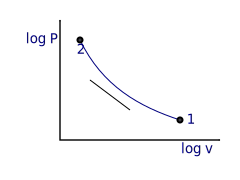
\includegraphics[width=40mm]{fig/nonExactPolytropic.pdf}
        \caption{A process displaying a curve in logarithmic $P\times v$ coordinates.}
        \label{fig:non.exact}
    \end{figure}

    Attempting to \emph{exactly} represent the process as a set of straight line segments  would
    result in an infinite set of segments, with each  one  being  of  vanishing  length---hence,
    having same end states. The definition of exact polytropic processes excludes all  processes
    in such a set from being exact polytropic ones; thus, the following Lemma:

    \begin{lemma}[continuously curved process]\label{lemm:curved.proc}
        A process whose path is continuously curved in $\log P \times \log v$ coordinates has no
        exact polytropic sub-process segments.
    \end{lemma}

    If, however, one allows for approximations, as is common practice in engineering, the curved
    process can be represented by  an  increasing  but  finite  amount  of  line  segments  with
    decreasing amounts of deviation (errors). The beginning of such  a  process,  in  which  the
    amount of line segments is doubled at each step, is depicted, with a shift in  $v$  for  the
    sake of improved visualization, on Figure~\ref{fig:approx}.

    \begin{figure}[ht]
        \centering
        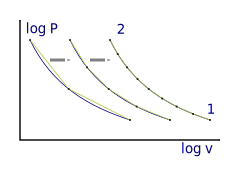
\includegraphics[width=40mm]{fig/approximations.pdf}
        \caption{Successive approximations to the curved process, in dark blue  solid  line,  by
            means of 2, 4, and 8 straight line  segment  sub-processes,  in  dark  yellow  solid
            lines,  in  $\log  P  \times  \log  v$  coordinates  (shifted  in  $v$  for   easier
            visualization)}
        \label{fig:approx}
    \end{figure}

    The rationale behind such approximation process is in support of the following definition:

    \begin{definition}[local polytropic process]\label{def:local.polytropic}
        A local polytropic process is a polytropic process that approximates or models a  subset
        of or another process to within suitable  error  intervals,  while  sharing  common  end
        states with it.
    \end{definition}

    Regarding  envisioned  capabilities  of  local  polytropic  processes  in  the  context   of
    equilibrium thermodynamics, one herein states:

    \begin{conjecture}[general approximability]\label{conj:gen.approx}
        Any continuous, quasi-equilibrium process set can be approximated or modeled, to  within
        finite error intervals, by a finite set of local polytropic processes.
    \end{conjecture}

    \begin{proof}[Remarks]
        It is worth noting that all equilibrium thermodynamic  \emph{cycles}  can  be  trivially
        subdivided into the process set stated on the general approximability conjecture,  since
        (sub-)process end states can be arbitrarily placed within the larger cycle path.
    \end{proof}

    The rationale behind the general approximability conjecture is the very definition of  local
    polytropic process, stated on Definition~\ref{def:local.polytropic}.

    Numerical methods in engineering typically employ a form of discretization of the underlying
    quantities. Numerical schemes geared towards solving equilibrium  engineering  thermodynamic
    cycles and processes may also apply the concept to \emph{processes}.

    \begin{proposition}[process modeling]\label{prop:proc.model}
        It is proposed that local polytropic processes, as herein defined,  to  be  employed  as
        discrete building blocks for  general  equilibrium  engineering  thermodynamics  process
        modeling.
    \end{proposition}

    A validated model description published by the author before the present formalization,  has
    successfully employed the proposed strategy  in  solving  Finite-Time  Heat-Addition  (FTHA)
    air-standard   Otto   cycles,   using   local   polytropic   processes   as    computational
    elements~\cite{2017-NaaktgeborenC-IntJMechEngEduc}.

    Since unsteady, non-instantaneous addition of heat in an  Otto  cycle  invariably  leads  to
    simultaneous heat and work interactions and result in non-trivial  thermodynamic  processes,
    even  under  quasi-equilibrium  hypotheses,  study~\cite{2017-NaaktgeborenC-IntJMechEngEduc}
    concluded that a set of discrete  polytropic  sub-processes  was  the  theoretical  tool  to
    provide the needed generality in the model  formulation,  and  thus,  inspired  the  current
    formulations.

%-----------------------------------------------------------------------------------------------
\section{Requisites for Exact Polytropic Processes}\label{sec:requisites}

    One can show that the polytropic relation, Equation~(\ref{eq:poly}), is the solution of
    %
    \begin{equation}
        \frac{dP}{P} = -n\frac{dv}{v},
        \label{eq:poly.ODE}
    \end{equation}
    %
    \noindent with $n$ not a function of either $P$ or $v$:
    %
    \begin{align}
        \int\frac{dP}{P} & = -n\int\frac{dv}{v} & \rightharpoondown
        \\
        \log P + \mathsf{c_1} & = -n\log v + \mathsf{c_2} & \rightharpoondown
        \\
        \log P & = -n\log v + \mathsf{c_3} & \rightharpoondown
        \\
        \log P + n\log v & = \mathsf{c_3} & \rightharpoondown
        \\
        Pv^n & = e^{\mathsf{c_3}} \equiv \mathsf{c},
    \end{align}
    %
    \noindent thus recovering Equation~(\ref{eq:poly}).

    The  work  of  Christians~\cite{2012-ChristiansJ-IntJMechEngEduc}  shows   that   internally
    reversible processes in closed systems with a calorically perfect gas  with  a  $Pv  =  ZRT$
    equation of state with constant compressibility factor $Z$ assuming  negligible  changes  in
    system kinetic and potential energies and constant energy transfer ratio,
    %
    \begin{equation}
        K \equiv \frac{\delta q}{\delta w},
        \label{eq:def.K}
    \end{equation}
    %
    \noindent yield a polytropic relation between $P$ and $v$ with a constant exponent $n = (1 -
    \gamma)K + \gamma$. In this work, $K$ is also referred  to  as  \emph{heat-to-work  transfer
    ratio}.

    The employed $Pv = ZRT$ equation of state is indicative of real gases; however, the constant
    $Z$ assumption narrows down the scope of the result. This prompts the  question  of  whether
    this finding is actually only applicable to ideal gases, for which $Z=1$, or  whether  other
    constants work.

    The energy balance equation for a closed system reads, in the intensive  differential  form,
    as
    %
    \begin{equation}
        \delta q - \delta w = du + de_k + de_p,
        \label{eq:1st.law.int.diff.micro.macro}
    \end{equation}
    %
    \noindent where $\delta q$ and $\delta w$ are the differential heat and  work  interactions,
    following the historical thermodynamic sign convention of positive heat  interactions  being
    into the system and positive work interactions being out of the system; $u$  is  the  system
    specific internal energy, with $e_k$  and  $e_p$  being  the  system  specific  kinetic  and
    potential (macroscopic) energies, respectively.  Neglecting  the  variation  of  the  system
    macroscopic  energy  forms,   simplifies   Equation~(\ref{eq:1st.law.int.diff.micro.macro}),
    giving:
    %
    \begin{align}
        \delta q - \delta w & = du, & \rightharpoondown
        \label{eq:1st.law.int.diff} \\
        (K-1)\delta w & = du,
        \label{eq:1st.law.int.diff.K}
    \end{align}
    %
    \noindent in which Equation~(\ref{eq:def.K}) is used.

    At  this   point,   reference~\cite{2012-ChristiansJ-IntJMechEngEduc}   replaces   $du$   by
    $c_v\,dT$---where $c_v$ and $c_p$ are the  constant-volume  and  constant-pressure  specific
    heats, respectively---in order to be able to arrive at a polytropic relation between $P$ and
    $v$, and continues the analysis with a $Pv = ZRT$ equation of state with the  assumption  of
    constant $Z$.

    Shortly after, the $ZR$ term is replaced by $(c_p - c_v)$, which can recover  an  ideal  gas
    result if $Z$ is further restricted to $1$. His analysis seems to request the adoption of an
    ideal gas model, rather than a real gas one, as the $ZR = (c_p - c_v)$ relation cannot  hold
    in general for a real gas. Take, for instance, the close vicinity  of  the  critical  state,
    predictable by a real gas model, in which $c_p \to +\infty$, even  if  approached  from  the
    monophase region, while all other quantities remain finite, indicating  the  $ZR  =  (c_p  -
    c_v)$ relation is subject to arbitrarily large errors in the real gas model domain.

    Moreover, from the perspective of real gas model, constant $Z$  in  general  must  be  based
    either on (i)~negligible reduced pressure, temperature, and specific  volume  variations  in
    the           process---recall           the           generalized           compressibility
    chart~\cite{2013-CengelYA+BolesMA-AMGH}---or on (ii)~the substance being in  the  ideal  gas
    limit during the entirety of the process.

    Following reference~\cite{2012-ChristiansJ-IntJMechEngEduc}, $du$ is replaced by  $c_v\,dT$,
    yielding a $u\!:\!u(T)$-only substance, whose property relations are  investigated.  In  the
    following, it is theoretically demonstrated  that  $Z\!:\!Z(v)$  for  such  a  substance---a
    useful intermediate result---among other outcomes.

    %---------------------------------------------------------------------------------------
    \subsection{Substance Equation of State Yielding $u\!:\!u(T)$}\label{sec:subst.eos}

    For $u\!:\!u(T)$ to hold, one must have:
    %
    \begin{equation}
        \parxyz uiT = 0.
        \label{eq:uT}
    \end{equation}
    %
    \noindent for \emph{any} choice of property $i$ other than $T$.

    Perhaps the easiest way of deriving the outcomes of Eq.~(\ref{eq:uT}) is by rewriting it  in
    terms of Bridgman's relations~\cite{2006-BejanA-Wiley}, which are expressed in  terms  of  a
    peculiar notation. Therefore, rewriting Eq.~(\ref{eq:uT}) in Bridgman's notation yields
    %
    \begin{equation}
        \frac{\bri uT}{\bri iT} \equiv \parxyz uiT = 0 \quad\rightharpoondown\quad \bri uT = 0.
        \label{eq:uT.bri}
    \end{equation}

    It is worth noting than the $\equiv$ sign on Eq.~(\ref{eq:uT.bri}) indicates the  definition
    of the \emph{ratio} between Bridgman's primitives $\bri  uT$  and  $\bri  iT$  in  terms  of
    $\inlxyz uiT$, rather than the other way around.

    Bridgman's relations are tabulated expressions for its \emph{individual primitives} in terms
    of    thermodynamic    properties    that    are    easily    obtainable    from    physical
    measurements~\cite{2006-BejanA-Wiley}, which makes them ingeniously useful.

    Bridgman's  peculiar  notation  allowed  Eq.~(\ref{eq:uT})  to  be  expressed  in  terms  of
    Bridgman's $\bri uT$ primitive only, thus eliminating  the  role  of  Bridgman's  $\bri  iT$
    primitive, \emph{irrespective of the choice of property $i$}. This  greatly  simplifies  the
    analysis of Eq.~(\ref{eq:uT})'s outcomes.

    From reference~\cite{2006-BejanA-Wiley}, one has
    %
    \begin{align}
        \bri uT & = v(\beta T - \kappa P) = 0 & \rightharpoondown \\
        \beta T & = \kappa P,
        \label{eq:bT.kP}
    \end{align}
    %
    \noindent where $\beta$ is the \emph{volumetric coefficient of thermal  expansion},  or  the
    \emph{volume  expansivity}~\cite{2006-BejanA-Wiley},  or  the  \emph{coefficient  of  volume
    expansion}~\cite{1986-JonesJB+HawkinsGA-Wiley},  and  $\kappa$   is   the   \emph{isothermal
    compressibility}~\cite{2006-BejanA-Wiley}, also denoted by some authors as $\kappa_T$, as to
    distinguish         it         from         the         isentropic          compressibility,
    $\kappa_s$~\cite{1986-JonesJB+HawkinsGA-Wiley}.

    Put differently, Eqs.~(\ref{eq:uT})--(\ref{eq:bT.kP}) indicate that any substance for  which
    $\beta T = \kappa P$ will have $u\!:\!u(T)$ only.

    Eq.~(\ref{eq:defs.aux}) brings forth definitions of $\beta$ and $\kappa$:
    %
    \begin{equation}
        \beta  \equiv \frac{1}{v}\parxyz vTP, \quad\mbox{and}\quad
        \kappa \equiv \frac{-1}{v}\parxyz vPT.
        \label{eq:defs.aux}
    \end{equation}

    Plugging  in  Eq.~(\ref{eq:defs.aux})  on  Eq.~(\ref{eq:bT.kP})   and   using   the   cyclic
    relationship,
    %
    \begin{equation}
        -1 = \parxyz ji\ell \parxyz\ell ji \parxyz i\ell j,
        \label{eq:cyclic}
    \end{equation}
    %
    \noindent gives, after some manipulation,
    %
    \begin{align}
        \parxyz TPv & = \frac{T}{P} & \rightharpoondown \\
        \left(\frac{\partial T}{T}\right)_{\!\!\!v} & =
            \left(\frac{\partial P}{P}\right)_{\!\!\!v} & \rightharpoondown \\
        T & = \mathsf{f}(v)P,
        \label{eq:uT.TPv}
    \end{align}
    %
    \noindent with $\mathsf{f}(v)$ arising from the partial integrations. Therefore, this result
    expresses a substance in which $T \propto P$  at  constant  volume.  Letting  $\mathsf{f}(v)
    \equiv f(v)/R$, yields
    %
    \begin{equation}
        Pf(v) = RT,
        \label{eq:uT.EoS}
    \end{equation}
    %
    \noindent with $f\!:\!f(v)$ being an arbitrary function of $v$ only.  If  this  equation  of
    state  is  represented  as  $Pv  =  ZRT$,  then  $Z  =  v/f(v)$,  as  previously  announced.
    Equation~(\ref{eq:uT.EoS}) is the most general equation of state for a  substance  that  has
    $u\!:\!u(T)$, and consequently $du = c_v\,dT$.

    %---------------------------------------------------------------------------------------
    \subsection{Specific Heats of a $u\!:\!u(T)$ Substance}\label{sec:specific.heats}

    Writing $s\!:\!s(T, v)$ and differentiating, with $du =  T\,ds  -  P\,dv$  and  the  Maxwell
    relation based on the Helmholtz energy, $\inlxyz svT = \inlxyz PTv$, one arrives at
    %
    \begin{equation}
        ds = \frac{c_v}{T}\,dT + \parxyz PTv\,dv.
        \label{eq:ds.Tv}
    \end{equation}

    Writing $s\!:\!s(T, P)$ and differentiating, with $dh =  T\,ds  +  v\,dP$  and  the  Maxwell
    relation based on the Gibbs energy, $\inlxyz sPT = -\inlxyz vTP$, one arrives at
    %
    \begin{equation}
        ds = \frac{c_p}{T}\,dT - \parxyz vTP\,dP.
        \label{eq:ds.TP}
    \end{equation}

    Equating  the  cross  derivatives  from  the  $dT$  and  $dv$  (or  $dP$)  coefficients   on
    Eqs.~(\ref{eq:ds.Tv}) and~(\ref{eq:ds.TP}), yields~\cite{2013-CengelYA+BolesMA-AMGH}:
    %
    \begin{align}
        \parxyz{c_v}vT & = +T\left(\frac{\partial^2P}{\partial T^2}\right)_{\!\!\!v},
        \quad\mbox{and}\label{eq:cv.test} \\
        \parxyz{c_P}PT & = -T\left(\frac{\partial^2v}{\partial T^2}\right)_{\!\!\!P}.
        \label{eq:cp.test}
    \end{align}

    Eqs.~(\ref{eq:cv.test}) and~(\ref{eq:cp.test}) are to be used  in  determining  whether  the
    specific heats of a substance with equation of  state  given  by  Eq.~(\ref{eq:uT.EoS})  are
    functions of other thermodynamic properties.

    Therefore, from Eq.~(\ref{eq:uT.EoS}), one has:
    %
    \begin{align}
        P & = \frac{RT}{f(v)} & \rightharpoondown \\
        \parxyz PTv & = \frac{R}{f(v)} & \rightharpoondown \\
        \left(\frac{\partial^2P}{\partial T^2}\right)_{\!\!\!v} & = 0.
        \label{eq:cv.test.0}
    \end{align}

    Therefore, $\inlxyz{c_v}vT = 0$ making $c_v\!:\!c_v(T)$ at best for a  Eq.~(\ref{eq:uT.EoS})
    substance.

    Let
    %
    \begin{equation}
        \mathsf{g}(v) \equiv f(v)/v.
        \label{eq:def.g}
    \end{equation}
    %
    \noindent then, from Eq.~(\ref{eq:uT.EoS}), one has:
    %
    \begin{align}
        v & = \frac{RT}{P\mathsf{g}(v)} & \rightharpoondown \\
        \parxyz vTP & = \frac{R}{P\mathsf{g}(v)} & \rightharpoondown
        \label{eq:vTP} \\
        \left(\frac{\partial^2v}{\partial T^2}\right)_{\!\!\!P} & = 0.
        \label{eq:cp.test.0}
    \end{align}

    Therefore, $\inlxyz{c_P}PT = 0$ making $c_P\!:\!c_P(T)$ at best for a  Eq.~(\ref{eq:uT.EoS})
    substance. Moreover, since
    %
    \begin{equation}
        \gamma \equiv \frac{c_p}{c_v},
        \label{eq:def.gamma}
    \end{equation}
    %
    \noindent one also has $\gamma\!:\!\gamma(T)$ at best for this substance.

    The textbook expression for $dh$ is~\cite{2013-CengelYA+BolesMA-AMGH}:
    %
    \begin{align}
        dh & = \parxyz hPT \,dT + \parxyz hTP \,dP \\
        dh & = c_p\,dT + \left[v - T\parxyz vTP \right]\,dP.
        \label{eq:dh}
    \end{align}

    From Eq.~(\ref{eq:vTP}), the $\inlxyz hTP$ term can be written as
    %
    \begin{align}
        \parxyz hTP & = v - T\parxyz vTP & \rightharpoondown \\
        \parxyz hTP & = v - \frac{RT}{P\mathsf{g}(v)} & \rightharpoondown \\
        \parxyz hTP & = v - v = 0,
        \label{eq:hTP}
    \end{align}
    %
    \noindent thus making $h\!:\!h(T)$ for a substance with $Pf(v) = RT$ equation of state.

    The findings of this subsection are thus summarized in an already proven theorem:

    \begin{theorem}[$u\!:\!u(T)$ substance]\label{theo:uT.subst}
        A substance for which $u\!:\!u(T)$, necessarily has $c_v\!:\!c_v(T)$,  $c_P\!:\!c_P(T)$,
        and $\gamma\!:\!\gamma(T)$ at best, and also $h\!:\!h(T)$. Moreover, it has a  $Pf(v)  =
        RT$ equation of state, with $f(v)$ being an arbitrary function of $v$.
    \end{theorem}

    %---------------------------------------------------------------------------------------
    \subsection{Energy Balance with a $u\!:\!u(T)$ Model}\label{sec:energy.balance}

    Plugging  in  $du  =  c_v\,dT$  on  Eq.~(\ref{eq:1st.law.int.diff.K})  and   differentiating
    Eq.~(\ref{eq:uT.EoS}) will make a $dT$ appear on both equations. Equating  the  common  $dT$
    leads to
    %
    \begin{equation}
        dT = \frac{K-1}{c_v}Pdv = \frac{Pf'(v)dv + f(v)dP}{R},
        \label{eq:dT.1st.law.EoS}
    \end{equation}
    %
    \noindent where $f'(v) \equiv df/dv$.

    The   goal   now   is   to   write   Eq.~(\ref{eq:dT.1st.law.EoS})   in    the    form    of
    Eq.~(\ref{eq:poly.ODE}), with constant $n$, which yields
    %
    \begin{align}
        \frac{dP}{P} & = - [f'(v) + (1 - K)(\gamma - 1)]\frac{dv}{f(v)}\quad\rightharpoondown\\
        \frac{dP}{P} & = -\frac{f'(v) + (1 - K)(\gamma - 1)}{\mathsf{g}(v)}\frac{dv}{v},
        \label{eq:Pv.ODE}
    \end{align}
    %
    \noindent in which $\mathsf{g}(v)$ is defined by Eq.~(\ref{eq:def.g}).  By  inspection,  the
    polytropic exponent is identified as:
    %
    \begin{align}
        n & \equiv \frac{f'(v) + (1 - K)(\gamma - 1)}{\mathsf{g}(v)} & \rightharpoondown
        \label{eq:n} \\
        n & = \frac{vf'(v)}{f(v)} + (1 - K)[\gamma(T) - 1]\frac{v}{f(v)}.
        \label{eq:n.deps}
    \end{align}

    The constancy of $n$ depends  on  the  constancy  of  all  of  Eq.~(\ref{eq:n.deps})  terms.
    Enforcing this condition upon the first term leads to the following ODE:
    %
    \begin{align}
        \frac{v}{f}\frac{df}{dv} & = \mathsf{c_1} & \rightharpoondown \\
        \frac{df}{f} & = \mathsf{c_1}\frac{dv}{v} & \rightharpoondown \\
        f(v) & = v^{\mathsf{c_1}} + \mathsf{c_2}.
        \label{eq:f.two.consts}
    \end{align}

    The second term of Eq.~(\ref{eq:n.deps}) contains $v$ and $T$ functions. Enforcing constancy
    separately in $v$ terms yields:
    %
    \begin{align}
        \frac{v}{f(v)} & = \mathsf{c_3} & \rightharpoondown \\
        \frac{v}{v^{\mathsf{c_1}} + \mathsf{c_2}} & = \mathsf{c_3},
        \label{eq:f.three.consts}
    \end{align}
    %
    \noindent which yields $\mathsf{c_1} = 1$, $\mathsf{c_2} = 0$, with $\mathsf{c_3} = 1$ being
    the only possibility for constancy in $v$ terms. This result  finally  fixes  the  substance
    equation of state by fixing $f(v)$ as
    %
    \begin{equation}
        f(v) = v.
        \label{eq:f}
    \end{equation}

    Consequently, the $Pf(v) = RT$ equation of state, with $f(v) =  v$,  \emph{exactly  recovers
    the ideal gas equation of state\/}, which reads
    %
    \begin{equation}
        Pv = RT.
        \label{eq:ideal.gas.EoS}
    \end{equation}

    Moreover, the constancy of the $(1 - K)[\gamma(T) - 1]$ term must account for the fact  that
    $K$ is defined only in terms of \emph{process  energy  interactions},  Eq.~(\ref{eq:def.K}),
    while  $\gamma(T)$  is  defined  only  in  terms  of  system  \emph{substance   properties},
    Eq.~(\ref{eq:def.gamma}). Therefore, the analysis is two-fold:

    (i)~For   interactions   that   yield   a   constant   value   of   $K$,   as   assumed   on
    reference~\cite{2012-ChristiansJ-IntJMechEngEduc}, one must have constant $\gamma(T) =  1  +
    R/c_v(T)$, for an ideal gas, which requires constancy in $c_v$, which, in turn,  also  means
    constancy in $c_p$, since $c_p = c_v + R$ for ideal gases.

    (ii)~For Eq.~(\ref{eq:n.deps})'s second term constancy, with $v/f(v) = 1$, interactions must
    be made system temperature dependent, i.e., $K\!:\!K(T)$, resulting in $[1 -  K(T)]  \propto
    c_v(T)$, which is hardly practical and is left as a note.

    Plugging the results back in  Eq.~(\ref{eq:n.deps}),  yields  the  value  of  the  resulting
    polytropic exponent:
    %
    \begin{equation}
        n = 1 + (1 - K)(\gamma - 1) = \gamma + K(1 - \gamma),
        \label{eq:n.final}
    \end{equation}
    %
    \noindent        which        is        in        agreement         with         Christian's
    results~\cite{2012-ChristiansJ-IntJMechEngEduc}.

    This section's outcomes are the base for the following, `K-polytropic', theorem:

    \begin{theorem}[K-polytropic]\label{theo:K.poly}
        Internally reversible processes in constant-specific-heat closed systems with negligible
        kinetic and potential energy changes and constant heat-to-work ratio interactions,  $K$,
        are exact polytropic processes only if the substance is an ideal gas.
    \end{theorem}

    Therefore, the  K-polytropic  theorem  answers  the  question  herein  raised  in  light  of
    Christian's    work~\cite{2012-ChristiansJ-IntJMechEngEduc},    that    the    constant-$Z$,
    $u\!:\!u(T)$ real gas working  substance  yielding  an  exact  polytropic  process  under  a
    reversible, constant-$K$ process in a closed system, needs to be further narrow down  to  an
    ideal gas, i.e., one for which $Z=1$.

%-----------------------------------------------------------------------------------------------
\section{Summary and Conclusions}

    This work has concerned  itself  with  polytropic  processes.  An  \emph{etymology}  of  the
    `polytropic' term  that  relates  to  its  mathematical  possibilities  has  been  given  on
    Section~\ref{sec:etymology}.

    The concept of a \emph{logical thermodynamic process}, idealized by the author as a  process
    with restricted end states, has been laid  out  by  Definition~\ref{def:logical.proc}.  With
    logical process, or logical conditions, processes and associated end states can be  uniquely
    referred to. Example~\ref{ex:ideal.Diesel} works out the concept on an  ideal,  air-standard
    Diesel cycle.

    The concept of \emph{exact polytropic process},  idealized  by  the  author  as  being  both
    logical, polytropic, and non-reversing, see Lemma~\ref{lemm:no.reversal}, has been laid  out
    in Section~\ref{sec:exact}. A  `Cycle'  theorem  relating  to  exact  polytropic  processes,
    Theorem~\ref{theo:cycle}, is provided. The way towards local  polytropic  process  is  paved
    with the discussion of processes  with  continuously  curved  paths  in  double  logarithmic
    $P\times v$ coordinates, see Lemma~\ref{lemm:curved.proc}.

    A definition of \emph{local polytropic process}, formulated  by  the  author---although  the
    concept of process relations applying locally is  found  in  previous  literature,  as,  for
    instance, in~\cite[p.~175]{2006-BejanA-Wiley}---that  explicitly  mentions  the  purpose  of
    approximation of another process, is provided  by  Definition~\ref{def:local.polytropic}  in
    Section~\ref{sec:local}.

    By means of the Conjecture~\ref{conj:gen.approx}, it is claimed  that  finitely  many  local
    polytropic process can be used to model \emph{any} given equilibrium thermodynamics  process
    or cycle to within finite  errors,  which  leads  to  Proposition~\ref{prop:proc.model},  of
    equilibrium thermodynamics numerical schemes to use them as  discrete  building  blocks  for
    general process modeling.

    A validated model description that employs discrete local polytropic processes  as  building
    blocks in general process modeling~\cite{2017-NaaktgeborenC-IntJMechEngEduc}, which has been
    published by the author before the present  formalization  of  concepts,  is  referenced  in
    Section~\ref{sec:local}      as      a      successful      case       in       implementing
    Proposition~\ref{prop:proc.model}.

    In Section~\ref{sec:requisites}, a statement  that  under  certain  conditions  a  gas  with
    $u\!:\!u(T)$ and a $Pv = ZRT$ equation of  state  with  constant  $Z$  displays  a  constant
    exponent   polytropic   process,   found   in~\cite{2012-ChristiansJ-IntJMechEngEduc},    is
    investigated using thermodynamic property relations, seeking theoretical requisites for  the
    occurrence of exact polytropic processes.

    Section~\ref{sec:subst.eos} shows that a $u\!:\!u(T)$ substance must  have  a  $Z\!:\!Z(v)$.
    Moreover, Section~\ref{sec:specific.heats} determines whether $c_v$,  $c_p$,  $\gamma$,  and
    $h$ of the $u\!:\!u(T)$ substance depend on properties other  than  $T$.  The  findings  are
    summarized in Theorem~\ref{theo:uT.subst}.

    It  is  finally  concluded,  in  Section~\ref{sec:energy.balance},  that  the  most  general
    $u\!:\!u(T)$ substance to yield an exact  polytropic  process  under  constant  heat-to-work
    transfer ratio is, in fact, an ideal gas---see Theorem~\ref{theo:K.poly}.

%-----------------------------------------------------------------------------------------------
\section*{Acknowledgments}

    This research received no specific grant from any funding agency in the public, private,  or
    not-for-profit sectors.

    To YHWH God be the glory!

%-----------------------------------------------------------------------------------------------

\bibliographystyle{plain}
\bibliography{bibfile}

%-----------------------------------------------------------------------------------------------
\end{document}
%-----------------------------------------------------------------------------------------------
